Nella precedente sezione \ref{subsec:supermercato24StrutturaArchitettura} è emersa la necessità di monitorare internamente il numero di ordini creati, consegnati, la loro distribuzione geografica e il fatturato totale in tempo reale.
A questi requisiti si sono aggiunti le informazioni riguardanti i clienti e un indice qualitativo del nostro servizio di consegna \verb+BOR+ (\textit{Bad Order Rate}).
Questo progetto è stato rinominato ``Socksberry'' dall'unione di ``Websocket'' e ``RaspberryPi''.

\subsection{Analisi iniziale}
\label{subsec:socksberryAnalisi}

\noindent
Le metriche \verb+KPI+ (\textit{Key Performance Indicator}) da analizzare e mostrare sono:
\begin{itemize}
  \item totale transato quotidiano
  \item conteggio degli ordini quotidiani
  \item conteggio degli ordini consegnati quotidiani
  \item conteggio degli ordini eliminati per inefficienza quotidiani
  \item conteggio degli accessi e registrazioni quotidiani
  \item latitudine e longitudine dell'indirizzo del cliente per ogni consegna
\end{itemize}

\bigskip
\noindent
Per ogni voce occorre poi estrarre:
\begin{itemize}
  \item valore record assoluto
  \item valore complessivo
  \item differenza percentuale rispetto al mese precedente
\end{itemize}

Tutti i valori dovranno essere aggiornati e calcolati in tempo reale senza appesantire il carico del \textit{server}.
L'output verrà mostrato su un monitor, tv o comunque dispositivi interni non smart tramite un browser.

\subsection{Implementazione}
\label{subsec:socksberryImplementazione}

Per poter estrarre tutti i dati e mantenerli congruenti si è preferito dividere il flusso in due fasi:
\begin{enumerate}
  \item fase di bootstrap, effettuata tramite query al Database
  \item fase di update, ad ogni ordine, del modello precedente tramite KeyValue
\end{enumerate}

Successivamente, si è preferito non esporre questo servizio sui \textit{server} di produzione per motivi di scalabilità e sicurezza.
Non è prevista nessuna policy di autenticazione, poiché viene garantita dalla comunicazione attraverso \verb+VPN+ con chiave \verb+RSA+.

Si è preferito utilizzare un \verb+RaspberryPi+ come elaboratore dati (\textit{``controller''}), il quale si connette al \textit{server} tramite una connessione \verb+VPN+ incapsulando le varie comunicazioni \verb+TCP+ verso il Database e verso il KeyValue instaurate da un applicativo \verb+NodeJs+.
Il software sviluppato, appena avviato, si connette al Database per ottenere i dati necessari (fase di ``bootstrap'') e successivamente instaura una comunicazione \textit{publish}/\textit{subscribe} (fase di ``update'') per ricevere gli aggiornamenti del modello.
Il programma è riportato in appendice \ref{app:socksberry_controller}.

\verb+RaspberryPi 3+ è un \textit{single-board computer} economico e portabile, costruito attorno ad un \verb+SoC+ (\textit{System-on-a-chip}).
Ospita un sistema operativo basato su kernel \verb+Linux+ e connesso alla rete aziendale tramite \verb+Wi-Fi+.
È stato installato: la piattaforma \verb+NodeJs+ per l'applicativo, \verb+Chromium+ come browser eseguibile a schermo intero da terminale e \verb+OpenVPN+ come terminatore della \verb+VPN+.

\begin{figure}[H]
  \centering
  \includegraphics[width=0.95\linewidth, keepaspectratio]{socksberry_uml}
  \caption{Modello delle connessioni del progetto Socksberry}
  \label{fig:socksberryUml}
\end{figure}

Per mostrare questi dati è stato sviluppato un applicativo \verb+Javascript+ (\textit{``view''}) collegato tramite \verb+HTTP+ \verb+WebSocket+ come descritto nella sezione \ref{subsec:httpWebsocket}.
La connessione \verb+HTTP+ asincrona permette di ricevere i dati solo quando disponibili, evitando aggiornamenti in un intervallo di tempo programmato.
Il programma è riportato in appendice \ref{app:socksberry_view}.

Si vengono a creare così due \textit{broker} distinti: il KeyValue che pubblica gli eventi del \textit{server} al \textit{controller} tramite connessione asincrona \verb+TCP+ e il \textit{controller} che pubblica gli eventi del KeyValue alla \textit{view} tramite connessione asincrona \verb+HTTP+.

\begin{figure}[H]
  \centering
  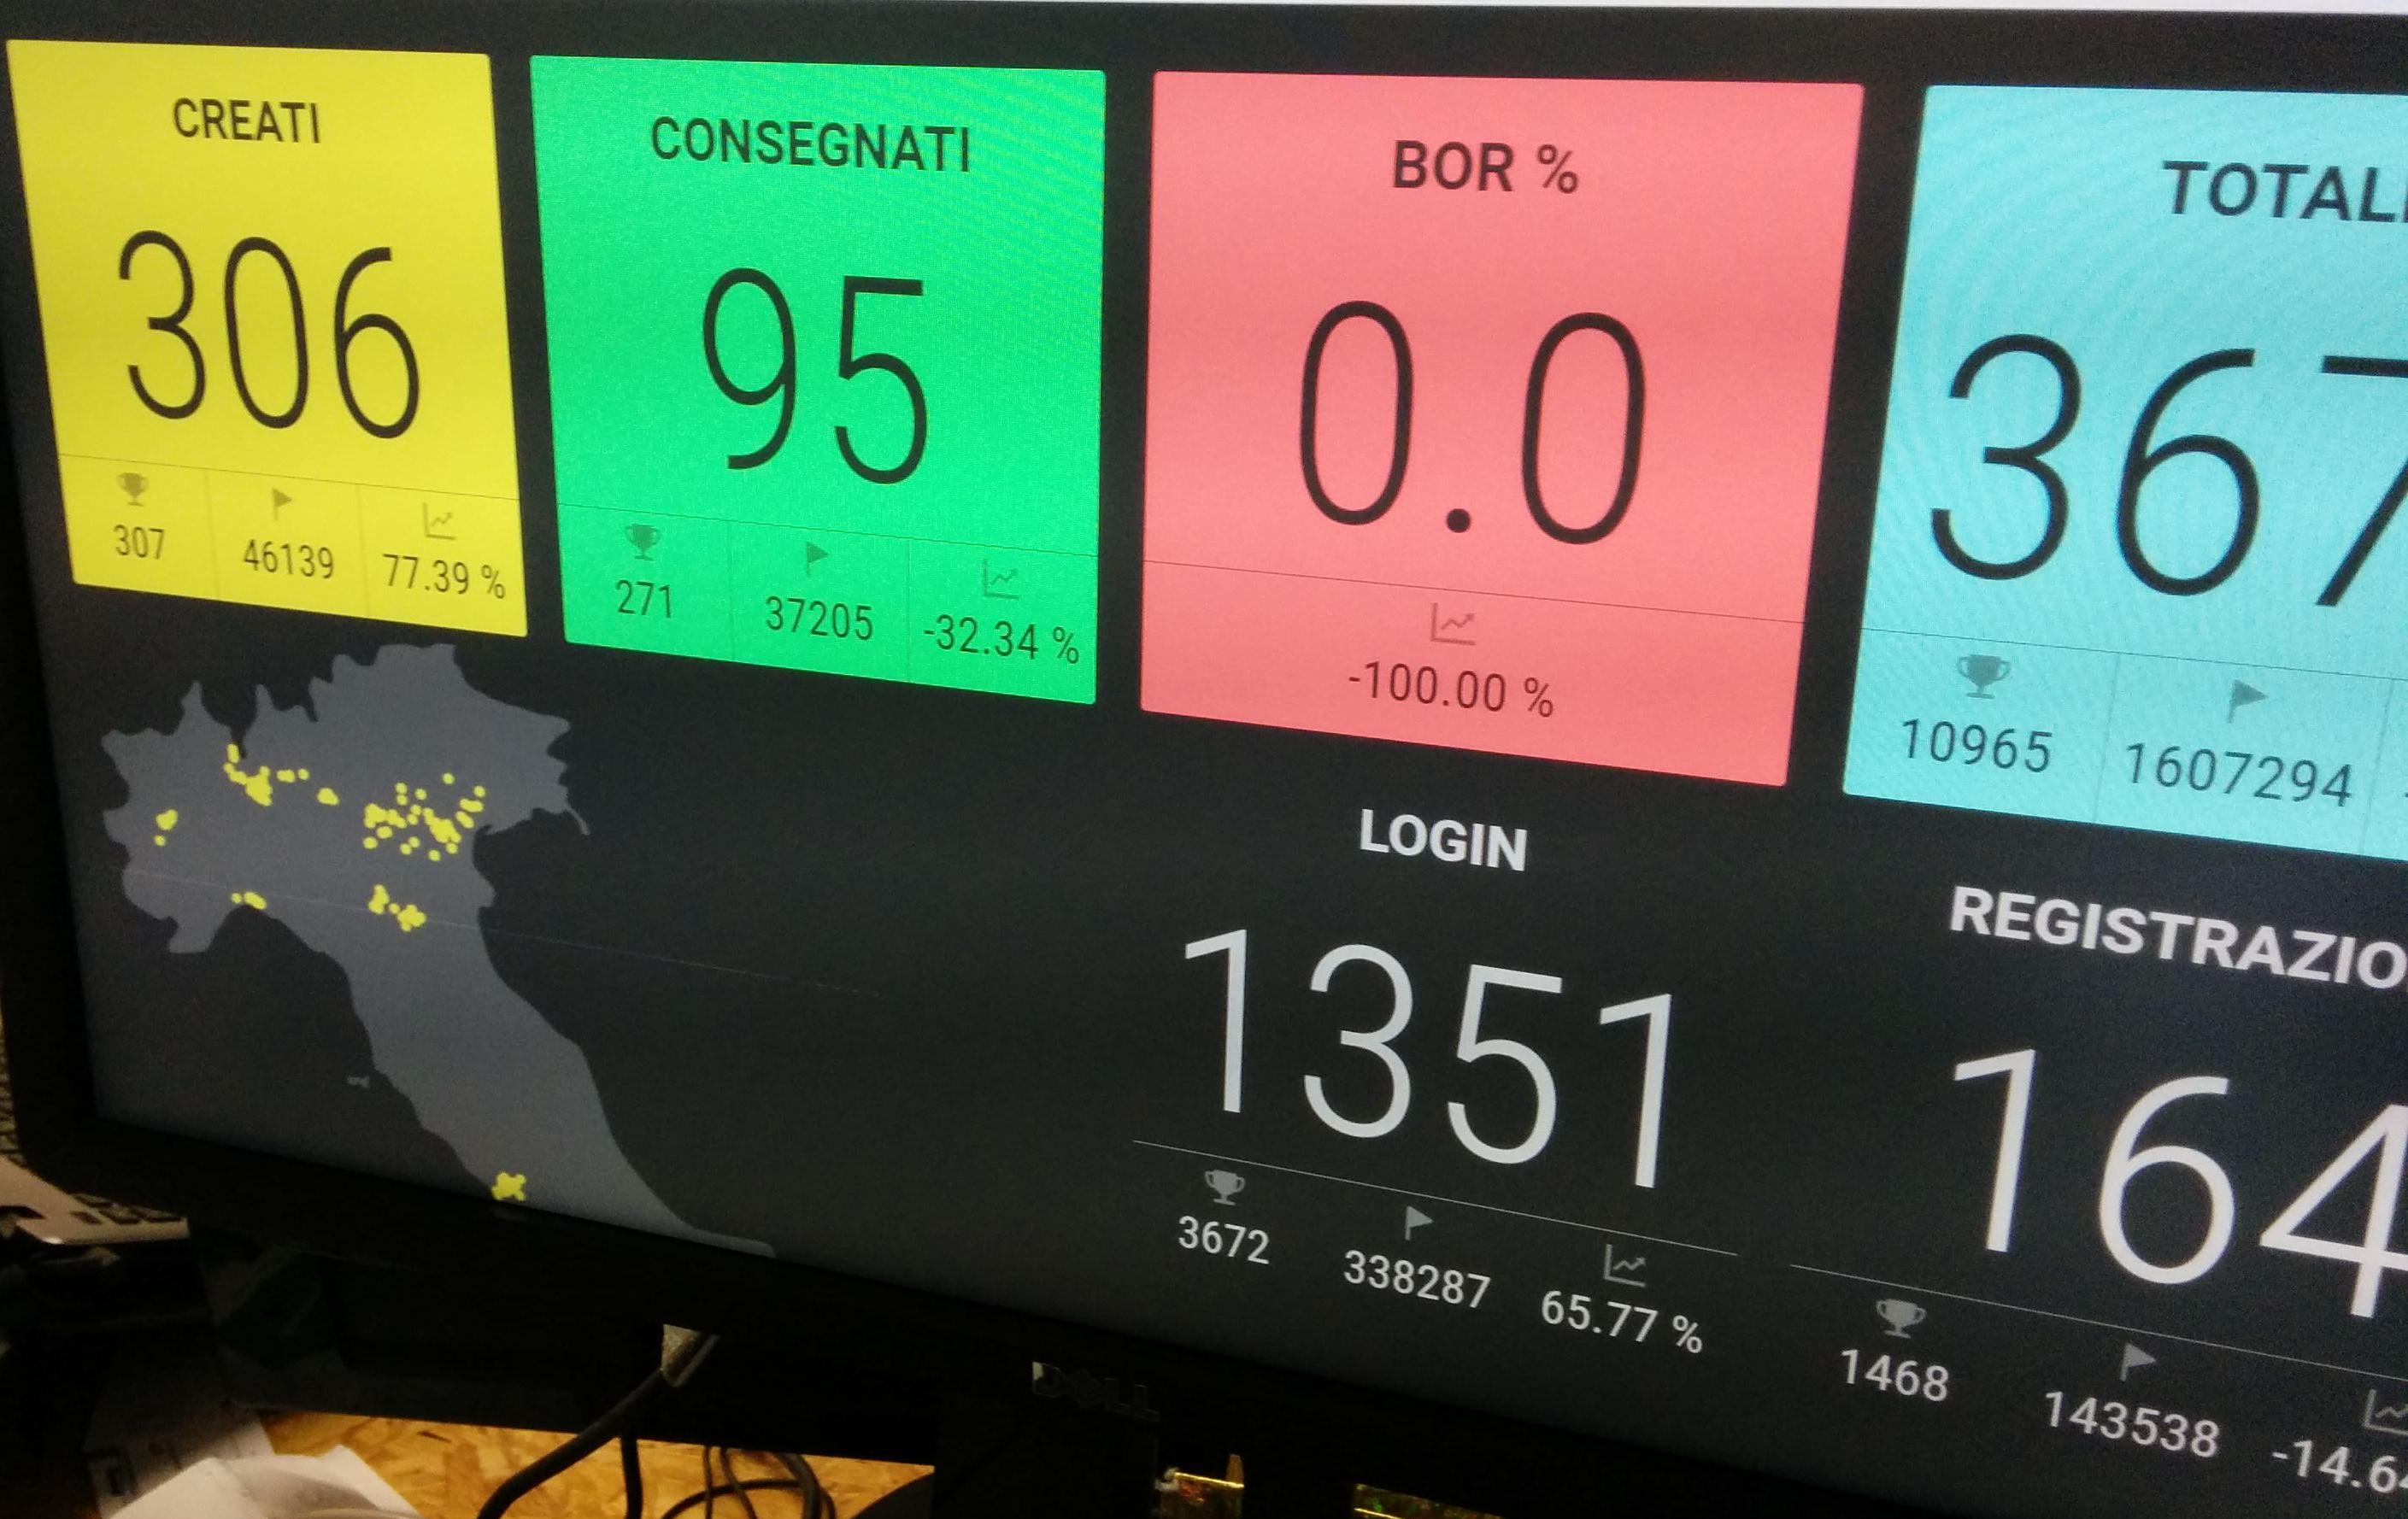
\includegraphics[width=0.95\linewidth, keepaspectratio]{socksberry_view}
  \caption{Foto del progetto Socksberry completato e operativo}
  \label{fig:socksberryView}
\end{figure}

\subsection{Difficoltà affrontate}
\label{subsec:socksberryDifficolta}

Inizialmente la fase di bootstrap dell'applicativo era associata alla prima connessione da parte di un \textit{client} e isolata da altri interlocutori.
Quindi per ogni \textit{client} connesso veniva effettuata una query iniziale e una \textit{subscription} dei \textit{topics} all'interno dello \textit{scope} del socket.
Si è poi reso necessario condividere questo modello tra tutti i socket, migliorando le performance e diminuendo il carico complessivo.

La comunicazione asincrona creata tramite \verb+WebSocket+ viene utilizzata prevalentemente in un'unica direzione: dal \textit{controller} verso la \textit{view}.
È stata proposta l'adozione dei \verb+SSE+, ma le notifiche non venivano inviate in tempo utile derivato dal delay progettuale.

La connessione da parte di un \textit{client} tramite \verb+WebSocket+ potrebbe venire effettuata mentre il \textit{controller} è in ancora in fase di bootstrap non ricevendo alcun dato e rimanendo inutilmente in attesa.
Abbiamo previsto, quindi, una fase ``init'' anche per la \textit{view}, aspettando la fase utile di scambio dati e attivando la grafica della \textit{dashboard} asincronamente.

\subsection{Conclusioni}
\label{subsec:socksberryConclusioni}

Si è scelto di non utilizzare il protocollo \verb+MQTT+ tra il \textit{controller} e la \textit{view} perché:
\begin{itemize}
  \item la batteria non è un fattore critico
  \item la banda non è un fattore critico
  \item la potenza computazionale non era condivisa con risorse critiche
  \item trattandosi di uno strumento di controllo interno non erano necessarie ottimizzazioni
\end{itemize}
